\documentclass[tikz,border=3pt]{standalone}
\usetikzlibrary{arrows.meta,calc}
\begin{document}
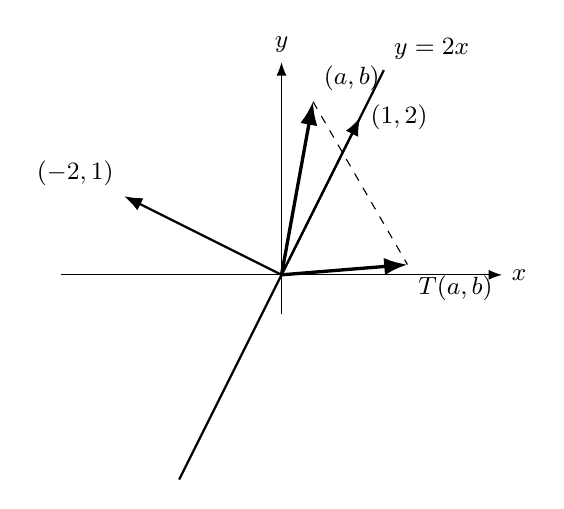
\begin{tikzpicture}[>=Latex, font=\small]
  \draw[->] (-2.8,0) -- (2.8,0) node[right] {$x$};
  \draw[->] (0,-0.5) -- (0,2.7) node[above] {$y$};
  \draw[thick] (-1.3,-2.6) -- (1.3,2.6) node[above right] {$y=2x$};

  \coordinate (P12) at (1,2);
  \coordinate (Pm21) at (-2,1);
  \coordinate (A) at (0.4,2.2);

  \draw[->, thick] (0,0) -- (P12) node[right] {$(1,2)$};
  \draw[->, thick] (0,0) -- (Pm21) node[above left] {$(-2,1)$};

  \draw[->, very thick] (0,0) -- (A) node[above right] {$(a,b)$};
  \draw[->, very thick] (0,0) -- (1.6,0.13) node[below right] {$T(a,b)$};
  \draw[dashed] (A) -- (1.6,0.13);
\end{tikzpicture}
\end{document}
